\documentclass{article}

\usepackage[utf8]{inputenc}

\usepackage{hyperref}
\usepackage{exercise}
\usepackage{amsmath}

\usepackage{graphicx}
\usepackage[siunitx]{circuitikz}

\usepackage{amsthm}
\newtheorem*{definition}{Definition}

\author{Mahdi Hasnat Siyam , 1705003}
\date{\today}
\title{Assignment on class note compilation (DSB-WC)}

\begin{document}

\maketitle

\section{Limitation of DSB-SC}
When demodulating a DSB-SC signal, the DSB-SC signal is multiplied by carrier frequency $\cos\left(\omega_ct\right)$. 
For demodulation, the receiver must generate a carrier in phase and frequency that was used during modulation.
This perfect match is not always possible. 

\section{The DSB-WC modulator}
We can solve this problem by sending carrier signal ($A\cos\left(\omega_ct\right)$) along with the modulated 
$m\left(t\right)cos\left(\omega_ct\right)$ signal. This type of modulator is called Double Side Band modulator - With Carrier (DSB-WC).
So transmitted signal is:
\begin{equation}
	\begin{split}
		T(t) &= m(t)\cos\left(\omega_ct\right) + A\cos\left(\omega_ct\right)
		\\
		&= \left(m(t)+A\right)\cos\left(\omega_ct\right)
	\end{split}
	\label{dsb-wc-equation}
\end{equation}
\section{Trade-off between DSB-SC and DSB-WC}


DSB-WC modulator needs to transfer carrier signal with the modulated signal.
So DSB-WC requires more power to transmit.

\smallskip
DSB-SC demodulator needs to multiply signals which is costly

\smallskip
In point-to-point (unicast) communication, there are a single sender and a single receiver. 
So using the DSB-SC modulator is not a problem.
But for communication with multiple points (broadcast), there are many receivers.
So using the DSB-WC modulator in this case, we can reduce the costs of receivers.
\smallskip
\begin{ExerciseList}
	\Exercise{For Broadcast communication which modulator should you use?}
\end{ExerciseList}

\section{Tone modulation}
\begin{definition}[Tone Signal]
	If the baseband signal is a sinusoid, it is called tone.
\end{definition}
Modulation done to a tone is known as tone modulation

\section{DSB-WC : Modulation}

From Equation \ref{dsb-wc-equation} modulated signal is:
\begin{equation*}
	T(t) = m(t)\cos\left(\omega_ct\right) + A\cos\left(\omega_ct\right)
\end{equation*}
In frequency domain, DSB-WC the modulated signal is:
\begin{equation*}
	T(\omega) = \frac{1}{2}M(\omega+\omega_c) + \frac{1}{2}M(\omega-\omega_c) +
	 \frac{A}{2}\delta(\omega+\omega_c) + \frac{A}{2}\delta(\omega-\omega_c)
\end{equation*}
Again from DSB-SC modulated signal in frequency domain is:
\begin{equation*}
	T(\omega) = \frac{1}{2}M(\omega+\omega_c) + \frac{1}{2}M(\omega-\omega_c) 
\end{equation*}
So modulated signal of DSB-WC in frequency domain is almost equal except two impulses at $\pm \omega$. 

\section{DSB-WC : Demodulation}
\subsection{Envelope}
Envelope of a signal is found by joining peaks of that signal.
\begin{figure}[h!]
	\centering
	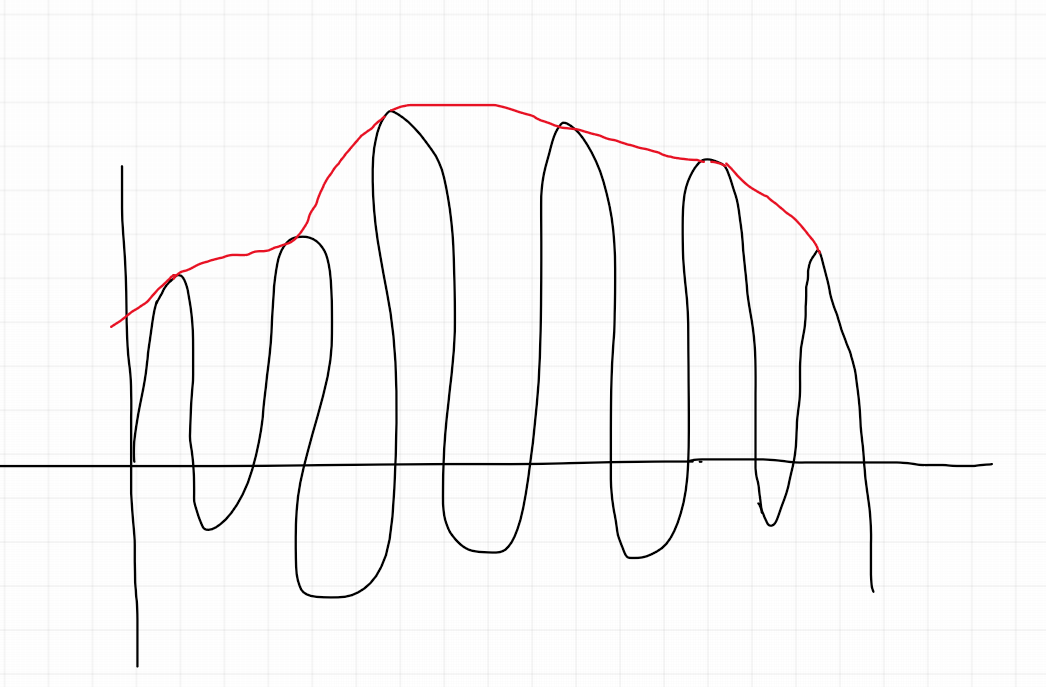
\includegraphics[scale=0.5]{images/envelope-hand_drawing.png}
	\caption{Here Red signal is the envelope of the black signal}
\end{figure}
\subsection{Envelope Detection}
If $m(t)+A$ is greater than $0$ for all $t$, 
then the envelope of the modulated signal is the modulated signal itself.
So we can detect the modulated signal by using envelope detection.
On the other hand if $m(t)+A$ is less than $0$ for any $t$, 
then envelope signal does not represent $m(t)$.


\begin{figure}[h!]
	\centering
	\begin{circuitikz}
		\draw
		(0,0) to[sinusoidal voltage source , l_ = $T(t)$]  (0,4)
		(0,4) to[diode] (4,4) 
		(4,4) to[] (7,4) node[below = 18mm](mt){$m(t)$} node[below](pls){+}
		(4,4) to[R,l_=$R$] (4,0)
		(6,0) to[C=C] (6,4)
		(0,0) to (7,0) node[above](mns){-}
		;
	\end{circuitikz}
	\caption{Envelope Detection Circuit}

\end{figure}
\subsection{Configuration of Circuit}
In envelope detection circuit, value of $R$, $C$ needs to be balanced for perfect demodulation.
If $RC$ value is vaery high, there will be slow discharge from capacitor and signal will be distored.
If $RC$ value is very low, there will be fast discharge and due to ripple effect intended $m(t)$ could not be recovered.
There are two options to balance $RC$ value.
\begin{itemize}
	\item Using current value of $RC$ to generate more accurate values of $R$ and $C$
	\item Changing value of $C$ such that following equation holds:
	\begin{equation*}
		\frac{1}{\omega_c} << RC < \frac{1}{2\pi B}
	\end{equation*}
\end{itemize}

\end{document}